\section{Unfolding}
%%%%%%%%%%%%%%%%%%%%%%%%%%%%%%%%%%%%%%%%%%%%%%%%%%%%%%%%%%%%%%%%%%%%%%
\label{sec:Unfolding}
In order to report the results in such a way that is easy to make a comparison with theoretical prescriptions or with other experiments results, the signal extracted performing the fit has to be corrected for detector resolution and efficiency effects and for the efficiency of the selection defined in the analysis.\\
To achieve this an unfolding procedure has been set up relying on the \textit{RooUnfold}~\cite{Adye:2011gm} package which provides the tools to run various unfolding algorithms.\\
The results are extrapolated to a fiducial region defined using generator level variables, as discussed in section \ref{sec:AnalysisStrategy}, in particular using  the status three definition for leptons, which identifies the ``hard part'' of the interaction, i.e. the partons that are used in the matrix element calculation, including immediate decays of resonances.
For this 8~\TeV analysis, in which the uncertainty is dominated by the low statistics, the effect of unfolding to status three particles (which are, strictly speaking, not observable) instead of status one (i.e. what one would observe with a perfect detector) are expected to be negligible.\\
The basic principle behind the unfolding procedure is to use MC signal samples to make the ``true'' distribution (the one obtained with MC truth information) of the variable of interest and the same distribution obtained with events reconstructed after the full GEANT4 simulation of the CMS detector and event reconstruction. These two distributions are used to calculate the response matrix $M$, given by:
\begin{equation}
R_i^{MC} = M_{ij}T_j^{MC} \quad ,
\end{equation}
where $R^{MC}$ and $T^{MC}$ are two n-dimensional vectors (where n is the number of bins of the distribution) representing the reconstructed distribution and to the true distribution respectively.\\
The response $M [n \times n]$ matrix includes all the effects related to the detector and to the analysis selection that affect the $R^{MC}$ distribution.\\
The goal of the unfolding procedure is to go back to the true distribution starting from the measured one. The most natural way to achieve this would be inverting the response matrix. However it can be shown~\cite{Cowan} that, due to the finite statistical accuracy of the response matrix, which is limited by the MC statistic, a simple inversion could lead to huge fluctuations between bins in the unfolded result. Regularization methods can however be employed to make the matrix inversion well behaved. Several methods are implemented in the RooUnfold package, and they all depend on the choice of a regularization parameter. The choice of the regularization parameter is particularly critical, and it should represent an optimal trade-off between taming the fluctuations in the unfolded result, and biasing the unfolded distribution towards the one used to build the response matrix. 

\subsection{Response matrix}
The first step is to build the response matrix.
The matrix is built as two-dimensional histograms, plotting the generator level Higgs \pt on the $x$ axis and the same variable at reconstructed level on the $y$ axis. For both the generator and reconstruction level variable the same binning has been chosen following the prescription described in section \ref{sec:Binning}.
Both fake events, i.e. events reconstructed in a given bin without a generated counterpart, and miss events, i.e. events generated in a given bin but not reconstructed, are taken into account in order to build the response matrix.
In figure \ref{fig:response_matrix} the response matrix is shown, either normalized by column or by row, in order to show respectively the purity and the stability values in the diagonal bins. The fake events distribution is shown in figure \ref{fig:fakes}. 
\begin{figure}[t]
\centering
\subfigure[]{
\includegraphics[width=0.45\textwidth]{images/response_matrix_newACC_purity.pdf}
}
\subfigure[]{
\includegraphics[width=0.45\textwidth]{images/response_matrix_newACC_stability.pdf}
}
\caption{Response matrix normalized to one either by column (a) or by row (b).}
\label{fig:response_matrix}
\end{figure}

\begin{figure}[b]
\centering
\includegraphics[width=0.6\textwidth]{images/fakes.pdf}
\caption{Fakes distribution, i.e. events reconstructed in a given bin without any generator level event associated, normalized to the data luminosity.}
\label{fig:fakes}
\end{figure}

\subsection{Regularization method}\label{sec:regularization}
In this analysis we used the SVD (Singular Value Decomposition) tool based on Tikhonov regularization function, provided within the \textit{RooUnfold} package. The choice of the regularization parameter follows the prescription in~\cite{Hocker:1995kb}. The prescription proceeds as follows: one needs to diagonalize the response matrix with the SVD decomposition and plot, as a function of the bin number, the values of a transformed vector called $d_{i}$ which represents the measured distribution in a specific base defined by the SVD decomposition. The optimal choice for the regularization parameter is a value that corresponds to where the curve becomes flat around 1.    
This choice is data driven and will have to be re-evaluated after the unblinding of the data. 
For the moment we have performed the test on the Monte Carlo, as shown in Fig.~\ref{fig:log_di}, and we decided to use a value of 3.
The test has been performed using 200 toy MC samples and calculating for each one of them the $\log{d_i}$ function. The values in each bin $i$ correspond to the mean values obtained from the toys and the corresponding errors.
However, the final choice of the regularization parameter has to be done looking at data after the unblinding.

\begin{figure}[htb]
\centering
\includegraphics[width=0.6\textwidth]{images/logdi_good.pdf}
\caption{Trend of the $\log{d_i}$ function as a function of $i$. The curve flattens for a value $i=3$, used as regularization parameter.}
\label{fig:log_di}
\end{figure}

In order to show the unfolded spectrum dependence on the choice of the regularization parameter, the unfolded procedure has been repeated for several regularization values. The various plots are shown in figure \ref{fig:kreg_test} for regularization values varying from 1 (stronger regularization) to 5 (weaker regularization). Using $k_{reg} = 6$ is equivalent to the simple inversion of the response matrix and leads to huge errors. Lowering $k_{reg}$ means increasing the regularization and thus reducing the statistical uncertainty. One should increase the regularization as much as possible until the procedure starts to bias the distribution. The distribution starts to be biased, according to the $\log{d_i}$ curve criterion, at $k_{reg} = 2$. Looking at figure \ref{fig:kreg_test}, the bias is clearly visible especially for $k_{reg} = 1$, when the unfolded distribution does not match anymore the MC truth.

\begin{figure}[htb]
\centering
\subfigure{
\includegraphics[width=0.45\textwidth]{images/kreg1.pdf}
}
\subfigure{
\includegraphics[width=0.45\textwidth]{images/kreg2.pdf}
}\\
\subfigure{
\includegraphics[width=0.45\textwidth]{images/kreg3.pdf}
}
\subfigure{
\includegraphics[width=0.45\textwidth]{images/kreg4.pdf}
}\\
\subfigure{
\includegraphics[width=0.45\textwidth]{images/kreg5.pdf}
}
\caption{Unfolded spectrum for several values of the $k_{reg}$ parameter, from 1 (stronger regularization) to 5 (weaker regularization).}
\label{fig:kreg_test}
\end{figure}

Another test that has been performed consists in unfolding a different distribution using the response matrix built with all the signal samples. The different measured distribution used for this test is obtained considering the VBF sample only. The results are shown in figure \ref{fig:VBF_test}, where the unfolded distribution is compared to MC truth, i.e. VBF sample only, for  four different values of the regularization parameter.\\
The plots show that the unfolded spectrum matches the MC truth only for high values of $k_{reg}$, while for lower values the unfolding procedure starts biasing the unfolded distribution, pushing it towards the spectrum used to build the matrix.
Of course this is a very extreme situation, where the measured spectrum is far from the expected one.

\begin{figure}[htb]
\centering
\subfigure[$k_{reg}=2$]{
\includegraphics[width=0.45\textwidth]{images/kreg2VBF.pdf}
}
\subfigure[$k_{reg}=3$]{
\includegraphics[width=0.47\textwidth]{images/kreg3VBF.pdf}
}\\
\subfigure[$k_{reg}=4$]{
\includegraphics[width=0.45\textwidth]{images/kreg4VBF.pdf}
}
\subfigure[$k_{reg}=5$]{
\includegraphics[width=0.47\textwidth]{images/kreg5VBF.pdf}
}
\caption{Unfolded spectrum for several values of the $k_{reg}$ parameter, from 2 (stronger regularization) to 4 (weaker regularization). The response matrix has been applied on top of a measured distribution containing the VBF signal only.}
\label{fig:VBF_test}
\end{figure}



\subsection{Closure test}\label{subsec:unfolding_closure}

A closure test has been performed in order to validate the unfolding procedure. For both gluon fusion and VBF, the samples have been splitted in two equal and statistically independent sets of events: the first set has been used to build the response matrix and the second one to construct the $p_\mathrm{T,gen}^\mathrm{H}$ distribution after the acceptance cuts only, i.e. the so called true distribution, and the $p_\mathrm{T,reco}^\mathrm{H}$ distribution after the full analysis selection, called measured distribution. The response matrix has then been applied on top of the measured distribution and the unfolded result has been compared with the true histogram. The results are shown in figure \ref{fig:unfold_test}. These plots show a nice agreement between the true histogram and the unfolded one within the uncertainties.
\begin{figure}[htb]
\centering
\includegraphics[width=0.7\textwidth]{images/closure_fakes.pdf}
\caption{Comparison among the measured distribution (blue markers), the unfolded distribution (red markers) and MC truth (green line). All signals (ggH, qqH and WZH) are included in the distributions.}
\label{fig:unfold_test}
\end{figure}

To estimate an uncertainty on the unfolding procedure due to the particular model adopted for building the response matrix we used two independent gluon fusion samples, obtained using two different generators: POWHEG (the default generator used in this analysis) and JHU. A comparison is shown in figure \ref{fig:jhu_powheg} between these two gluon fusion samples for the Higgs \pt spectrum normalized to unity.
\begin{figure}[htb]
\centering
\includegraphics[width=0.7\textwidth]{images/jhu_powheg.pdf}
\caption{Comparison between the generator level \pth spectra obtained with POWHEG and JHU for the gluon fusion production mode.}
\label{fig:jhu_powheg}
\end{figure}
The JHU gluon fusion sample has been used to build the response matrix and the POWHEG sample to extract the true and the measured histograms to be compared with the unfolded distribution. The results are shown in figure \ref{fig:jhu_powheg_unfold} and, as can be observed, we have a nice agreement between the true and the unfolded histograms.\\
\begin{figure}[htb]
\centering
\includegraphics[width=0.7\textwidth]{images/jhu_powheg_unfold.pdf}
\caption{Closure test in which the JHU ggH sample has been used to build the response matrix and the POWHEG sample to extract the true and measured distributions.}
\label{fig:jhu_powheg_unfold}
\end{figure}

As a further cross check we have evaluated the effect of changing the relative fraction of VBF and ggH within the theoretical uncertainty. The test is shown in Fig.~\ref{fig:vbfOverGghRatioVaried}, where three different response matrices, for the nominal, scaled up and scaled down VBF/ggH ratio have been used to unfold the reconstructed level distribution obtained with the nominal VBF/ggH ratio.
\begin{figure}[htb]
\centering
\includegraphics[width=0.7\textwidth]{images/gghvbfratio.pdf}
\caption{Unfolded distributions for the nominal ggH/VBF ratio (black line) and the scaled up (red line) and down (blue line) distributions.}
\label{fig:vbfOverGghRatioVaried}
\end{figure}


%\subsection{Signal unfolding}\label{subsec:signal_unfolding}

%As discussed in section \ref{sec:SignalExtraction}, we divided all the sources of uncertainties in two categories: the uncertainties correlated across bins and the ones that are not.
%The strategy is to unfold in a different way this two kind of sources. The part of the uncertainty including the statistical contribution and the effect of uncorrelated nuisances has been extracted fitting an Asimov toy dataset and removing all the correlated nuisances. In this way we get the effect of this kind of source on the signal strengths in each bin. At this point the postfit results are divided into the ggH and the VBF (including also the other production modes) contributions and used to build the measured $p_T^H$ spectra. These distributions are unfolded using the matrices built as explained before.\\
%The effect of each correlated nuisance on signal strength has been evaluated producing the same ggH and VBF distributions but changing the nuisance prefit nominal value by $1~\sigma$ up and down. Each up and down variation is unfolded separately in order to take properly into account the correlation between the nuisances.\\
%Among the correlated nuisances there are some that have an effect also on the response matrix. For these systematic uncertainties up and down variations an ad hoc response matrix has been made and used for unfolding them.
%The shape systematics that affect the response matrix are: b-tagging uncertainty, leptons efficiency, MET resolution, MET scale variation and electron resolution. Leptons scales do not change the response matrix because the variation of the electron or muon scale manifests as a similar variation of the MET scale but in the opposite direction (follows from the MET definition), resulting in a cancellation of the two effects. Jets energy scale variation also has no effect on the response matrix, because the $p_T^H$ definition is unrelated to jets' variables.\\

\subsection{Comparison to ZZ and $\gamma\gamma$ approach}
We have followed an unfolding procedure that is different from what has been
done in similar differential analyses in ZZ and $\gamma\gamma$. In those
analyses the correction for bin migration is done at the fit level, by
defining the signal according to the truth level binning, rather than the
reco-level binning. Then one applies a selection efficiency correction.

We have tried the same approach, obtaining the fit result in
Fig.~\ref{fig:embedded_unfolding} (a). The large errors obtained seem to
indicate a substantial equivalence between this method and an un-regularized
matrix inversion (Fig.~\ref{fig:embedded_unfolding} (b)), although we haven't
investigated mathematically this equivalence further. Since our response
matrix is significantly non-diagonal, regularization is needed to avoid large
statistical errors.

\begin{figure}[htb]
\centering
\subfigure[]{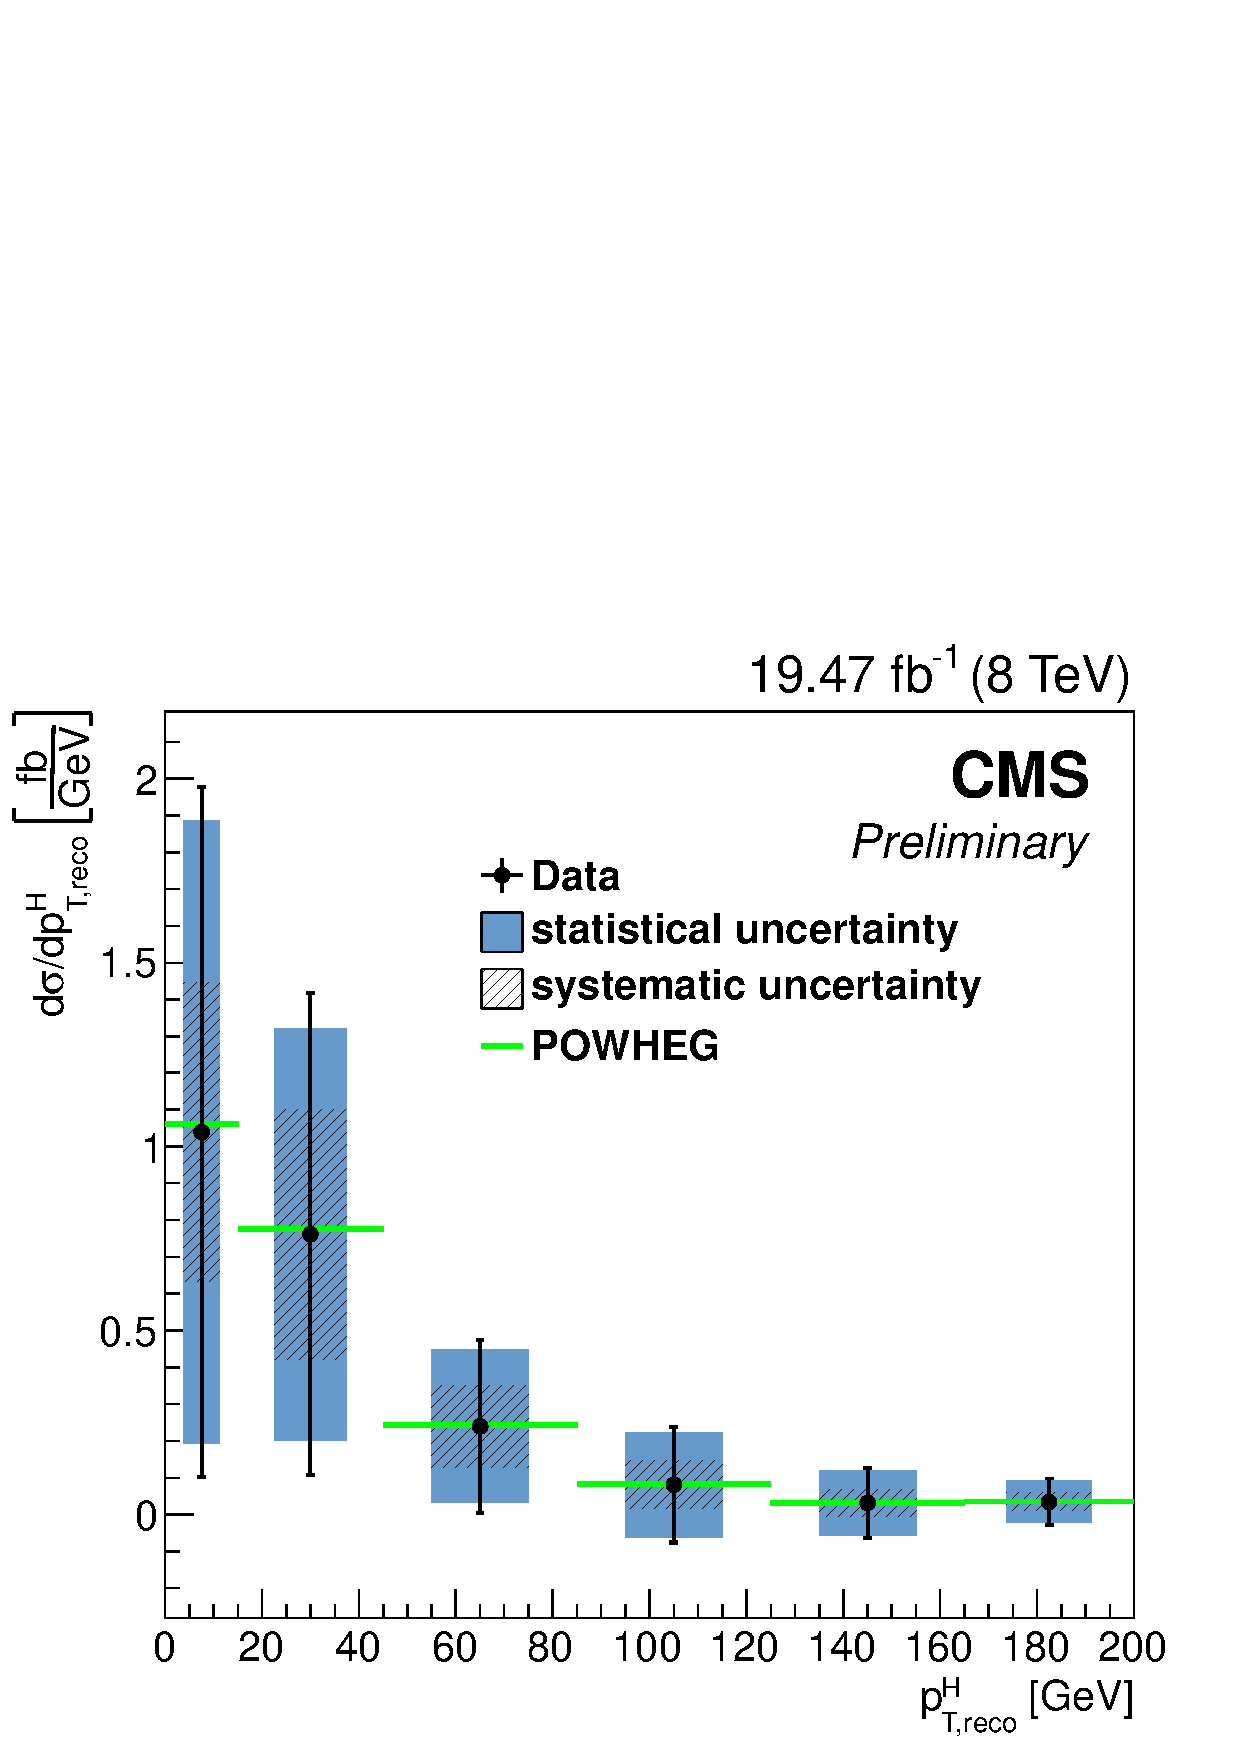
\includegraphics[width=0.45\textwidth]{images/embedded_unfolded.pdf}}
\subfigure[]{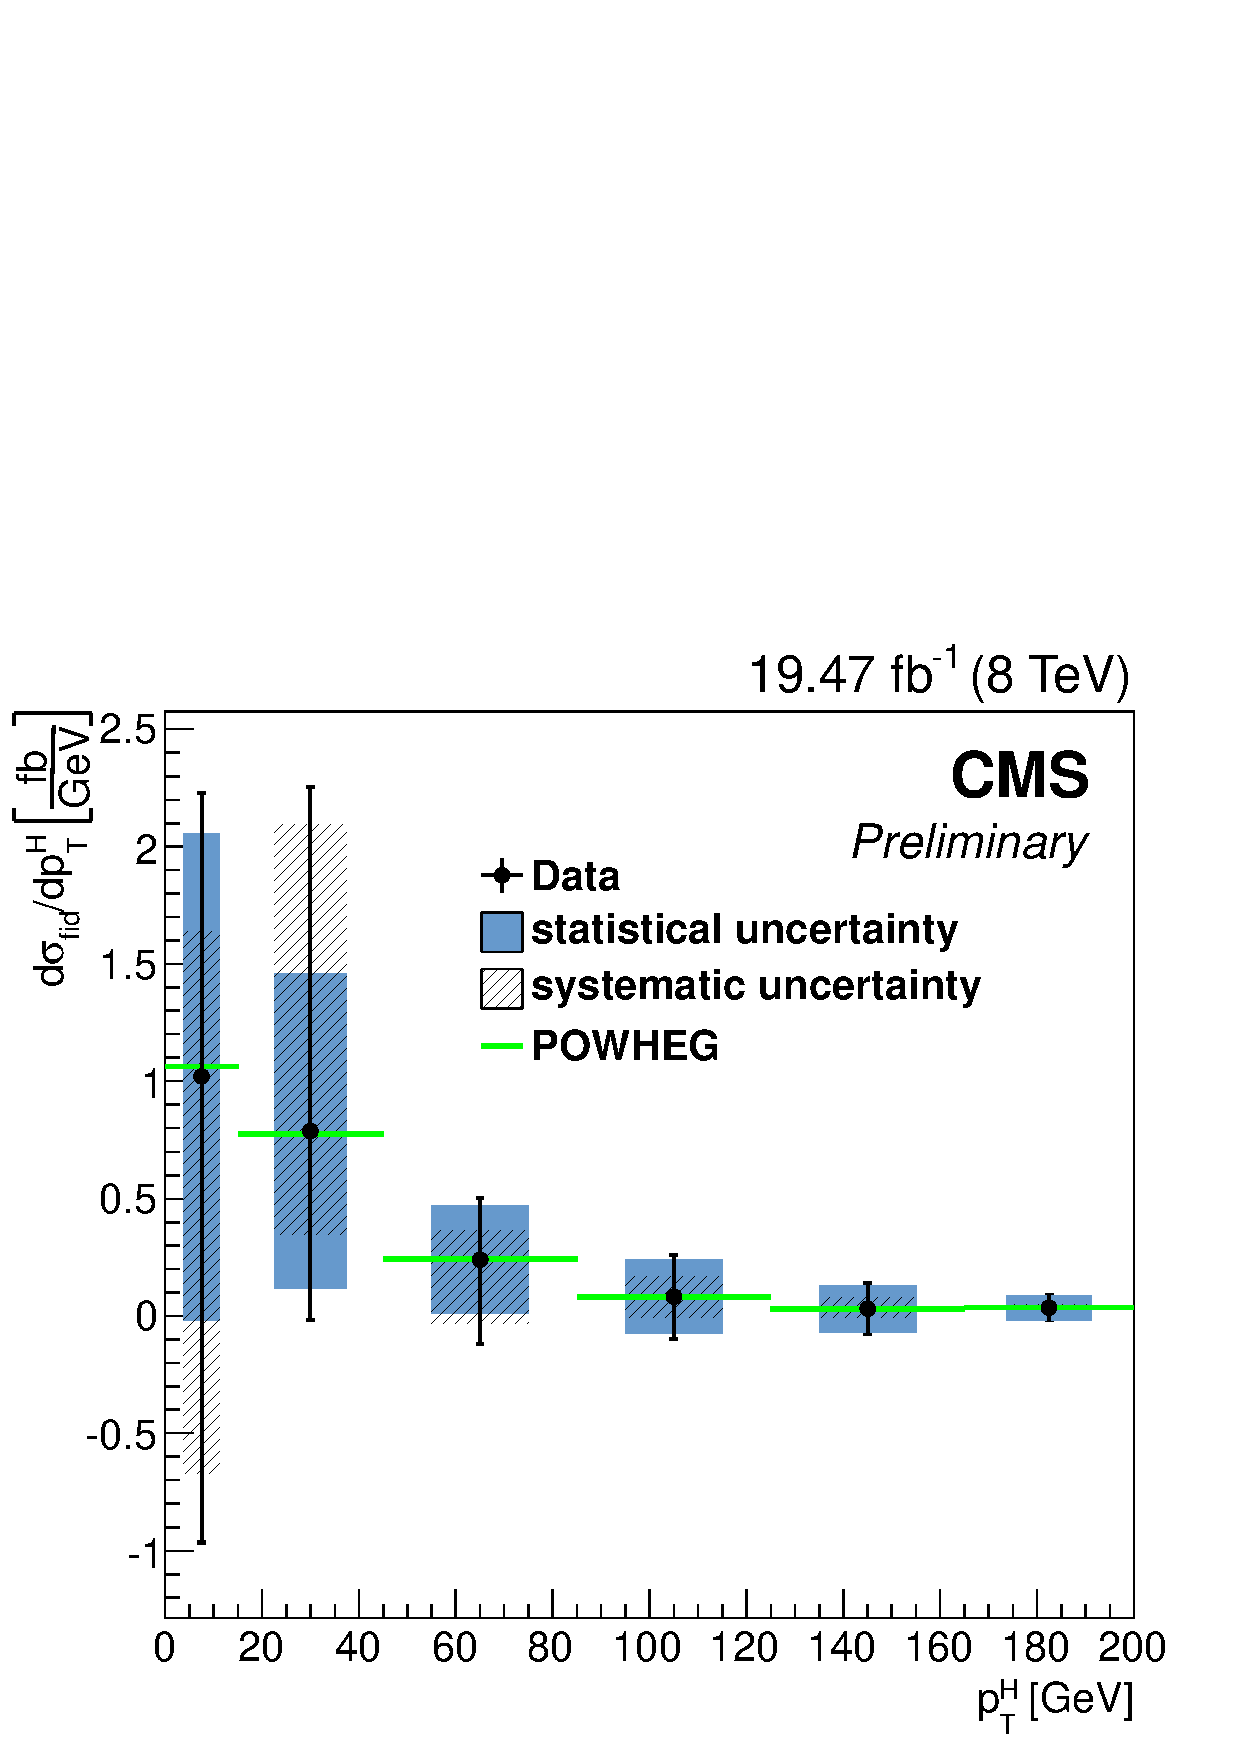
\includegraphics[width=0.45\textwidth]{images/unfolded_invert.pdf}}
\caption{(a) extraction of the un-smeared signal yields from the fit as in
differential ZZ and $\gamma\gamma$. (b) Plain matrix inversion with regular
fit.\label{fig:embedded_unfolding}}
\end{figure}



